\chapter{Definition Logging, Tracing {\fontfamily{bch}\selectfont \&} Monitoring}\label{ch:definition-von-logging-tracing-&-monitoring}
\textcolor{blue}{
    \enquote{Die perfekten IT-Systeme, die zuverlässig und ohne Fehler ihre Dienste tun, gibt es nicht. Ein funktionierendes IT-System ist kein Zustand, sondern ein Prozess, der von Menschen (Administratoren) permanent begleitet werden muss.}}\autocite{cloudradar}.
Logging zeichnet auf, was eine Anwendung macht.
Tracing protokolliert, wenn eine Anwendung andere Services aufruft.
Monitoring zieht aus diesen Informationen Schlüsse, um Fehler einer Anwendung aufzudecken.
Wenn die gefundenen Fehler korrigiert werden, kommt man dem fehlerfreien System näher.
Im Folgenden werden die drei Verfahren genauer erklärt.


\section{Logging}\label{sec:logging}
Als Logging wird das automatische Protokollieren von Ereignissen bezeichnet.
Hierzu zählen Fehlermeldungen, Systemnachrichten, Statusmeldungen, etc.
Die Daten, die protokolliert werden, werden in eine oder mehrere Log-Dateien geschrieben.
Diese Dateien enthalten die Ereignisse mit Zeitstempel, welche meist chronologisch geschrieben werden.\autocite{ip-insider}
\\
Außerdem werden die einzelnen Logs mit einem Loglevel versehen, womit der Entwickler das Protokoll besser auswerten kann.
Es gibt sechs verschiedene Loglevel.
Durch das gesetzte Loglevel können die Logs in einem Protokoll nach diesem Parameter gefiltert werden.
Hierfür muss eine einheitliche Struktur der Logs gewährleistet sein.
\textcolor{blue}{
    Die Logs haben die Struktur: Datum, Uhrzeit, Loglevel, Thread, Klassenname und Nachricht.}
\\
\begin{figure}[!h]
    \centering
    \textcolor{blue}{
        \begin{itemize}
            \item Fatal:
            \begin{itemize}
                \item Logs spiegeln wider, dass die Applikation in einem katastrophalen Zustand ist und eingegriffen werden muss
                \item es sollte sofort eingegriffen werden, um die Applikation wieder verfügbar zu machen
            \end{itemize}
            \item Error:
            \begin{itemize}
                \item Applikation ist auf einen Fehler getroffen, läuft trotzdem weiter
                \item Administrator sollte so schnell wie möglich untersucht werden
            \end{itemize}
            \item Warning:
            \begin{itemize}
                \item Applikation ist einem Zustand, der nicht üblich ist
                \item sollte analysiert werden, um den Normalzustand wiederherzustellen
                \item Fehler hat nicht höchste Priorität, da die Anwendung weiter läuft
            \end{itemize}
            \item Information
            \begin{itemize}
                \item Level wird hauptsächlich in produktiven Umgebungen genutzt
                \item wird genutzt, um Aktivitäten der Anwendung nachvollziehen zu können
            \end{itemize}
            \item Debug
            \begin{itemize}
                \item wird in Testumgebungen genutzt
                \item stellt weitere Informationen zur Auswertung bereit
            \end{itemize}
            \item Verbose
            \begin{itemize}
                \item alle Details einer Anwendung werden dokumentiert\autocite{ait}
            \end{itemize}
        \end{itemize}}\label{fig:figure4}
\end{figure}
\\
\\
\\
Das Log-Management kümmert sich um die langfristige Speicherung, sodass die Daten über lange Zeit nachvollziehbar sind.
Hierbei sollten die Logs an einer zentralen Stelle gespeichert werden, wie zum Beispiel einer Datenbank.
Logs sollten bestimmten Standards entsprechen, um die Integration mit zentralisierten Protokollierungsdiensten zu erleichtern.
Die Logs können kurzfristig auch in der Konsole ausgegeben werden, können dadurch aber nicht langzeitig ausgewertet.
Lokale Speicherung der Logs in Dateien erschweren das Auswerten.\autocite{ip-insider, ait}
\\
Das Event-Management stellt Funktionen bereit, um diese Daten auswerten zu können.
Zusammengefasst Log- und Event-Management sammeln die Log-Daten, speichern sie, sodass die Daten genutzt werden können, um Probleme zu identifizieren, Prozesse nachzuvollziehen, Systemleistung zu optimieren oder Cyberangriffe und andere Sicherheitsvorfälle zu erkennen und abzuwehren.\autocite{ip-insider}
%TODO: Visualisierung
\\
\\
Logs helfen dabei Sicherheitsvorfälle zu identifizieren.
Falls gegen Richtlinien verstoßen wird, fallen diese in den Logs durch die Überwachung auf.
In den Protokollen werden Informationen festgehalten, um Probleme und ungewöhnliches Verhalten nachvollziehen zu können.
\\
Manche Logs sind durch den Gesetzgeber verpflichtend, um Ereignisse nachverfolgen zu können.
Transaktionen im Bankumfeld sind verpflichtend aufzuzeichnen, um die Nachvollziehbarkeit dieser Aktionen sicherzustellen.
Im Gesundheitswesen ist Logging gesetzlich gefordert, um Compliance-Richtlinien zu erfüllen.
Unter anderem gilt die Datenschutzgrundverordnung \textcolor{blue}{DSGVO}, um \textcolor{blue}{personenbezogene} Daten richtig zu verarbeiten.\autocite{ip-insider, owasp}
\\
\\
Durch künstliche Intelligenz
\textcolor{blue}{
    können große Datenmengen organisiert werden.
    Maschinelles Lernen ermöglicht Daten automatisiert auswerten.
    Hierfür werden historische Daten genutzt, um Algorithmen zu entwickeln, die zum Auswerten genutzt werden.
}\autocite{ip-insider}
\\
\\
Logging sollte innerhalb einer Anwendung einheitlich verwendet werden.
Das Logging sollte in der gesamten Organisation konsistent verwendet werden, um die Ereignisse, die in den Protokollen abgelegt sind, mit Ereignissen verschiedener Systeme vergleichen und verwalten zu können.
\\
\textcolor{blue}{
    Log Events} können aus verschiedenen Quellen \textcolor{blue}{stammen.
Bei einer }
Client-Software, können die Interaktionen auf dem Desktop oder dem mobilen Gerät aufgezeichnet werden.
Bei der Nutzung einer Datenbank sollten jeder Aufruf protokolliert werden.
Zum Beispiel das Auslesen, Verändern oder Löschen eines Datensatzes sollte als Ereignis im Protokoll aufgenommen werden.
Falls vertrauliche Daten abgelegt sind, müssen diese auch vertraulich in den Logdateien abgelegt sein.
Der Vertraulichkeitsgrad muss beibehalten werden, um die Daten weiterhin zu schützen.
\\
Um die Sicherheitsstandards, die Alarmierung und Berichterstattung von Logausgaben zu erfüllen, müssen das Niveau und der Inhalt in der Anforderungsanalyse und Entwurfsphase entwickelt und festgehalten werden.
Niveau und Inhalt sollte in einem angemessenen Verhältnis zu dem Informationsrisiko stehen.
Hierfür gibt es keine einheitliche Checkliste, da jedes Unternehmen, Organisation und Anwendung verschieden sind.\autocite{owasp}
\\
\\
Jeder Eintrag in einem Protokoll muss \enquote{wann, wo, wer und was} aufzeichnen.
\textbf{Wann} steht hierbei für den Zeitstempel des Ereignisses mit Datum und Uhrzeit in einem internationalen Format.
Dieser kann vom Protokollierungszeitpunkt abweichen.
\textbf{Wo} steht für die Kennung der Anwendung, beispielsweise der Name und die Version.
Die Anwendungsadresse sollte auch protokolliert sein, hierzu zählt die IP-Adresse und Portnummer des Servers.
\textbf{Wer} ist aufgeteilt in menschlicher und maschineller Benutzer.
Zum einen die Quelladresse, beispielsweise die IP-Adresse des Benutzers oder die Mobiltelefonnummer.
Zum anderen die Benutzeridentität, falls dieser authentifiziert ist, zum Beispiel der Benutzername oder die Lizenznummer.
\textbf{Was} steht für die Schwere des Ereignisses, also dem Loglevel, und die Beschreibung des Ereignisses.
Weitere mögliche Aufzeichnungen sind HTTP-Statuscodes oder interne Einordnung.
\\
Manche Ereignisse dürfen nicht direkt in die Protokolle geschrieben werden.
Sie müssen gesondert behandelt werden, entweder entfernt, maskiert, gehasht oder verschlüsselt werden.
Daten wie Quellcode, sensible Informationen oder Authentifizierungskennwörter gehören zu diesen besonders zu behandelnden Ereignissen.
Verschlüsselungsschlüssel und andere Geheimnisse müssen geschützt werden.
Inhaberdaten von Bankkonten und Zahlungskarten müssen besonders geschützt gespeichert werden.
Anders zu behandeln sind Daten wie Dateipfad, interne Netzwerkdaten oder nicht sensible personenbezogene Daten.
Hierfür muss die Organisation selbst entscheiden, wie sensibel diese Daten protokolliert werden sollen.\autocite{owasp}
\\
\\
Nach Möglichkeit sollten Fehler bei der Eingabevalidierung in den Logs gespeichert werden.
Authentifizierungserfolge und -fehler sollten protokolliert werden.
Zugriff sollte kontrolliert werden und Autorisierungsfehler sollten geloggt werden.
Anwendungsfehler und Systemereignisse, beispielsweise wie Laufzeitfehler oder Verbindungsprobleme, sollten im Protokoll gespeichert werden.
Um Anwendungen und verwandte Systeme zu überwachen, sollte jeder Start und Stop aufgezeichnet werden.
Optional sollten weitere Ereignisse protokolliert werden, um die Sicherheit einer Anwendung zu erhöhen.
Übermäßiger Gebrauch sollte dokumentiert sein.
In den Protokollen sollte verdächtiges oder unerwartetes Verhalten einer Anwendung oder eines Systems erkennbar sein.\autocite{owasp}
\\
\\
Die Protokolle mit den gesammelten Ereignissen müssen nach dem Speichern vor Missbrauch geschützt werden.
Beispielsweise müssen Daten vor unbefugten Zugriff bewahrt werden.
Manche Protokolle enthalten Daten, die der Konkurrenz dienen können.
Geschäftliche Werte können Journalisten von Nutzen sein, um Schätzungen über Einnahmen zu machen.\autocite{owasp}


\section{Tracing}\label{sec:tracing}
Ein Trace ist die direkte Visualisierung eines Requests beim Durchlauf durch eine Anwendung oder eine komplette Anwendungslandschaft.
Tracing macht es möglich, nachzuvollziehen, in welchen Zuständen ein Objekt zuvor war.
Allerdings erhöht Tracing die Komplexität des Codes und ist daher besser geeignet für Microservicearchitekturen.
Ein Trace zeichnet die verschiedenen Aufrufe auf, beispielsweise einen HTTP-Request oder einen Datenbankaufruf.
Während der Entwicklung einer Anwendung können Zusatzinformationen zum Verarbeitungsprozess nützlich sein.
Neben den üblichen Ausgaben einer Anwendung helfen die Zusatzinformationen beim Testen der Anwendung.\autocite{adesso}
\\
\\
Bei Microservices hilft das Distributed Tracing, es bezeichnet die verteilte Rückverfolgung.
Hierbei werden einzelne Prozesse getrennt und somit wird erkennbar, wo Probleme entstanden sind.
Um bei Problemen den verursachenden Microservice zu identifizieren, erhält jeder Prozess eine Profil-ID.
Jeder Microservice signiert jede Nutzungsanfrage mit dieser ID.
Alle Prozesse lassen sich so einem bestimmten Service zuordnen, identifizieren und analysieren.
Falls nun ein Fehler auftritt, lässt sich der Microservice, der den fehlerhaften Prozess ausführt, durch die ID identifizieren.
Insgesamt ist die Fehlersuche vereinfacht.
Des Weiteren unterstützt Tracing beim Debugging.\autocite{adesso,dotnet,dev-insider}
\\
\\
Tracing wird in verschiedenen Arten spezifiziert.
Im allgemeinen Gebrauch für Anwendungen wird als Trace der Aufruf anderer Systeme bezeichnet.
Während der Pandemie haben wir das ortsbezogene Tracing kennengelernt.
Hierbei ist ein Trace die Nachverfolgung eines bestimmten Ereignisses, beispielsweise der Besuch einer Gastronomie.
Außerdem gibt es das nähebezogene Tracing.
Hierfür werden die Personen bzw\. deren Geräte nachverfolgt und geschätzt wer, wie nah und wie lange in der Nähe war.\autocite{monstarlab}
\\
\\
Oft wird Tracing mit Tracking verglichen oder sogar verwechselt.
Der Unterschied liegt dabei, dass Tracking den aktuellen Zustand beschreibt, wie zum Beispiel die GPS-Koordinaten einer Bestellung.
Tracing beschreibt das Nachverfolgen, für das gleiche Beispiel wird beim Tracing der Bestelleingang, Verarbeitungsprozess etc\. protokolliert.
\textcolor{blue}{Tracing beschreibt die Vergangenheit und Tracking beschreibt den aktuellen Zustand eines Objektes.}\autocite{monstarlab}


\section{Monitoring}\label{sec:monitoring}
Monitoring sammelt viele Daten und zielt darauf ab, richtige Schlüsse zu ziehen.
Ein einfaches Beispiel, das Monitoring sollte erkennen, dass ein Problem vorliegt, wenn eine Komponente ausfällt.
Hierfür wird die Anwendung konstant überwacht und der Status aller Komponenten erfasst.
Des Weiteren werden die Daten der Anwendung oder Systems aufbereitet und bewertet, sodass sie in einer übersichtlichen Zusammenfassung präsentiert werden können.
Durch Monitoring fallen Abweichungen vom Normalzustand auf, dadurch sollte ein Alarm ausgelöst werden, um den Nutzer aufzufordern den Fehler zu beheben.
Je nach Schweregrad des Fehlers werden verschiedene Medien zum Benachrichtigen des Nutzers verwendet.
Bei schweren Fehlern kann eine SMS auf das Arbeitstelefon geschickt werden.
Bei leichteren Fehlern kann eine Email reichen.\autocite{cloudradar, crossmedia}
\\
\begin{figure}[!h]
    \centering
    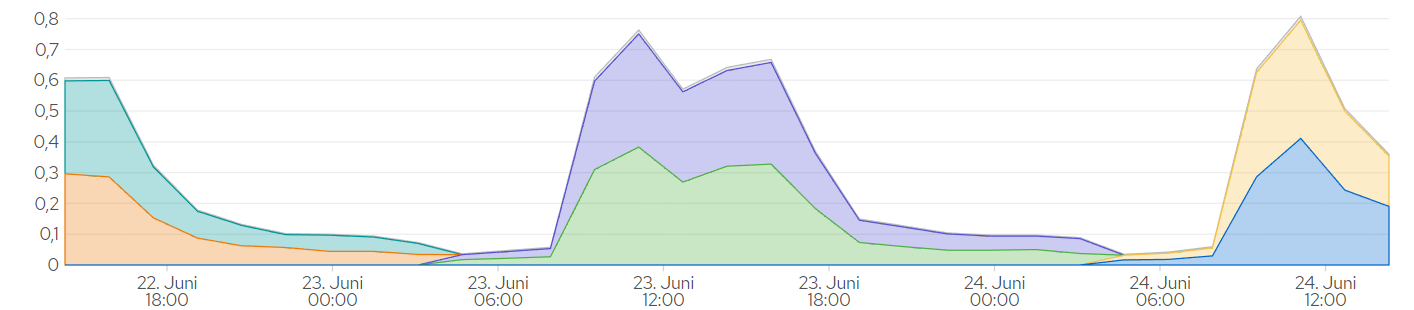
\includegraphics[width=\linewidth]{images/cpu-ozv-web2}
    \caption{CPU-Auslastung über 2 Tage}\label{fig:figure}
\end{figure}
\\
\\
\textcolor{blue}{
    Die Abbildung~\ref{fig:figure} zeigt die CPU-Auslastung über 2 Tage.
    Es ist zu erkennen, dass die Auslastung tagsüber während den regulären Arbeitszeiten wesentlich höher ist als nachts.
}
\\
\\
Durch den Vergleich zu historischen Daten soll das Monitoring-System Aussagen über die Zuverlässigkeit einer Anwendung treffen.
Durch das Überwachen einer Anwendung können Ausfälle vermieden und vorgebeugt werden.
Ein User-Interface des Monitorings zeigt die Performance und Auslastung der Komponenten, die durchgehend gemessen werden.
Diese Überwachung wird genutzt, um Hardwareausstattung zu planen.\autocite{cloudradar}
\\
\\
Monitoring bietet viele Vorteile.
Zum Einen werden die Abhängigkeiten zwischen Anwendungen abgebildet.
Zum Anderen werden Trendanalysen genutzt, um den Einsatz von Rechenleistung und Ressourcen zu verbessern.
\textcolor{blue}{Des Weiteren wird nicht nur das Endprodukt sondern jede Teilkomponente überwacht.
Außerdem werden Ressourcenengpässe frühzeitig erkennbar gemacht.}\autocite{wbs, cloudradar}
\\
\\
Monitoring ist in zwei Arten vorhanden.
\\
Einmal gibt es das \enquote{Historical Monitoring}, welches proaktives Arbeiten fordert.
Hierbei muss der Admin vorausschauend das Handeln planen.
Mit Langzeitstatistiken werden Kapazitäten geplant und können die Budgetplanung des Unternehmens unterstützen.
Der Admin erkennt die Missstände, informiert die Betroffenen und entwirft Lösungsansätze.
\\
Die zweite Art des Monitoring ist das \enquote{Real-Time-Monitoring}.
Hierbei werden die Server überwacht und bei Problemen direkt reagiert.
Im Idealfall werden Fehler registriert und behoben, bevor der Nutzer diesen bemerkt.\autocite{crossmedia}
\\
\\
Anforderungen an ein Monitoring-System können in fünf Kategorien unterteilt werden.
\\
\begin{figure}[!h]
    \textcolor{blue}{
        \begin{itemize}[noitemsep]
            \item Zustand des Systems
            \begin{itemize}
                \item \enquote{End-to-End}-Monitoring: überprüft Daten so nah wie möglich am Endnutzer auf Funktionalität
                \item Statuserfassung der Dienste, unter anderem Hardwareauslastung und Softwareüberwachung
                \item Informationen für lange Zeit speichern, um die Verfügbarkeit von Diensten und Komponenten analysieren
            \end{itemize}
            \item Alarmierung
            \begin{itemize}
                \item fordert das manuelle Eingreifen
                \item Mitarbeiter wird über die Fehlerursache informiert
                \item Reaktionszeit und Fehlerbehebung wird dokumentiert
            \end{itemize}
            \item Diagnose
            \begin{itemize}
                \item Informationen werden gesammelt, um die Ursachenanalyse von Fehlern detailliert zu ermöglichen
                \item die gesammelten Informationen dienen der Entscheidungsfindung
            \end{itemize}
            \item Qualitätsmessung
            \begin{itemize}
                \item Daten werden gesammelt, die über die Leistungsfähigkeit und den Durchschlag von Systemen und Anwendungen Aufschluss geben
                \item vereinbarte Grenzwerte und deren Einhaltung wird erfasst
                \item Engpässe und Überlastungen werden aufgedeckt
            \end{itemize}
            \item Konfiguration
            \begin{itemize}
                \item standardisierte Konfigurationen überwachen
                \item bei Abweichungen von standardisierten Vorgehen warnen \autocite{cloudradar}
            \end{itemize}
        \end{itemize}\label{fig:figure5}}
\end{figure}

%\section{Sinnvolle Nutzung}\label{sec:sinnvolle-nutzung}
%\section{Sinnvolle Ausgaben}\label{sec:sinnvolle-ausgaben}
%\section{Wann ist es übertrieben?}\label{sec:wann-ist-es-übertrieben?}
